\section{Results}
\label{results_section}

We followed the methods explained in \cref{methods_section} to create a new dataset and run the models listed \cref{model_selection} in order to measure their knowledge grounding of each one of these models when adding counterparametric context.

This section presents the results from these runs.

\subsection{Creating a representative dataset of questions}
\label{dataset_results}

As described in \cref{questions_objective} and explained in \cref{creating_dataset}, we require a new and diverse dataset in order to run this data and answer the research question.

We manually create a set of 4760 questions using the method explained in \cref{creating_dataset}.

In order to be able to reuse objects for different questions, we separated the questions and objects in 9 different categories.

\begin{enumerate}
	\item \textbf{Person} Historical people living from early antiquity to the present day from all around the globe. The questions have short, unambiguous answers, such as date of birth or most famous invention.
	\item \textbf{City} Cities from all over the globe. Questions may include population, founding date, notable landmarks, or geographical features.
	\item \textbf{Principle} Scientific principles, discovered from the 16th century forward. Questions about their discovery, use, and others.
	\item \textbf{Element} Elements from the periodic table. Questions may cover discovery, atomic number, chemical properties, or common uses.
	\item \textbf{Book} Literary works from various genres, time periods, and cultures. Questions may involve authors, publication dates, plot summaries, or literary significance.
	\item \textbf{Painting} Famous artworks from different art movements and periods. Questions may cover artists, creation dates, styles, or current locations.
	\item \textbf{Historical Event} Significant occurrences that shaped world history, from ancient times to the modern era. Questions may involve dates, key figures, causes, or their historical consequences.
	\item \textbf{Building} Notable structures from around the world, including ancient monuments, modern skyscrapers, and architectural wonders. Questions may cover location, architect, construction date, or architectural style.
	\item \textbf{Composition} Musical works from various genres and time periods. Questions may involve composers, premiere dates, musical style, or cultural significance.
\end{enumerate}

Each one of these categories has a number of questions that are assigned one of the objects, following and enhancing the question-building approach used by \citeauthor{factual_recall}.

The final list of base questions and objects for all categories can be found in \cref{appendixA}.
The total amount of these and composition of the 4760 questions can be found in \cref{category_amounts}.

\begin{table}[ht]
	\centering
	\scriptsize
	\begin{tabular}{>{\bfseries}l r r r}
		\toprule
			\bfseries Category & \bfseries Base Questions & \bfseries Objects & \bfseries Total Questions \\
		\midrule
			Person           &  17 &  57 &  969 \\
			City             &  17 &  70 & 1190 \\
			Principle        &   5 &  37 &  185 \\
			Element          &  15 &  43 &  645 \\
			Book             &  11 &  49 &  539 \\
			Painting         &  12 &  44 &  528 \\
			Historical Event &   4 &  64 &  256 \\
			Building         &   9 &  22 &  198 \\
			Composition      &  10 &  25 &  250 \\
		\midrule
			Total            & 100 & 411 & 4760 \\
		\bottomrule
	\end{tabular}
	\caption{The amount of base questions, objects, and the total amount of questions in each category on the final dataset after merging the base questions with the objects of each respective category.}
	\label{category_amounts}
\end{table}

\subsection{Building an experimental framework to understand the source of an LLM's answer}
\label{parametric_vs_contextual}

\subsubsection{Building and running the framework}
\newcommand{\somecode}[1]{\fcolorbox{Gray!80}{Gray!40}{\ttfamily #1}}

The code used for running this framework is present in \cref{appendixD}.
This code roughly follows the diagram on \cref{action_diagram} to run the following steps.
\begin{enumerate}
	\item Generate questions from base questions and objects: \somecode{combine\_questions}.
	\item Gather the parametric answers for each model: \somecode{QuestionAnswerer.answerChunk}.
	\item Shuffle them to create counterfactual answers: \somecode{sample\_counterfactual\_flips}.
	\item Build new queries with these counterfactual answers as context: \somecode{Question.format}.
	\item Run the models again, and gather the corresponding answer type for each answer from the results: \somecode{QuestionAnswerer.answerCounterfactuals}.
\end{enumerate}

The models were run on a server with 48 Intel(R) Xeon(R) CPU 3GHz CPUs, 376GB of RAM, and 2 NVIDIA A100 GPUs with 80GB of VRAM each that was kindly provided to Artificial Intelligence MSc students in City, University of London.

We estimate that it's possible to run this framework for all but the largest model, \texttt{Meta-Llama-3.1-70B}, using a single A100 GPU.

\Cref{appendixC} explains the many options that can be run on \texttt{knowledge\_grounder.py} to re-run this experiment or run similar ones.

\subsubsection{Framework Results}
\label{framework_results}

The results of running the queries created in \cref{creating_dataset} with added counterparametric context on each of the four models the four models can be found in \cref{total_table,total_results}.

\begin{table}[htbp]
	\centering
	\scriptsize
	\begin{tabular}{l r r r}
		\toprule
			\bfseries Model & \Parametric{} & \Contextual{} & \Other{} \\
		\midrule
			\smallflan{}  & 248 & 4284 & 228 \\
			\bigflan{} & 242 & 4304 & 214 \\
		\midrule
			\smallllama{} & 745 & 3662 & 353 \\
			\bigllama{} & 1070 & 3303 & 387 \\
		\bottomrule
	\end{tabular}
	\caption{Amount of answers of each category when running our dataset on each of the four models. Seq2Seq models tend to generate using the parametric context more often than Decoder-only models, while for the latter the size of the model makes a large difference.}
	\label{total_table}.
\end{table}

\begin{figure}[ht]
	\centering
	\subfigure[Seq2Seq models]{
		\raggedleft
		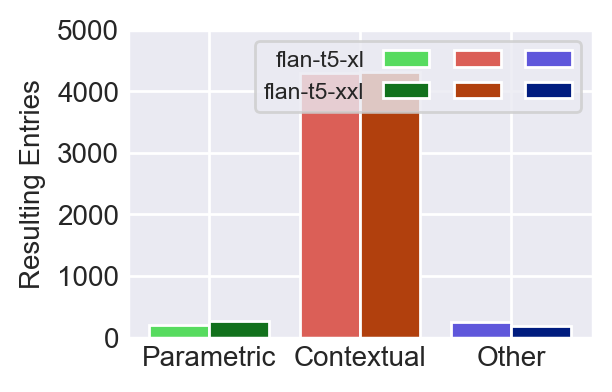
\includegraphics[width=.42\textwidth]{flan_amount.png}
	}%
	\subfigure[Decoder-only models]{
		\raggedright
		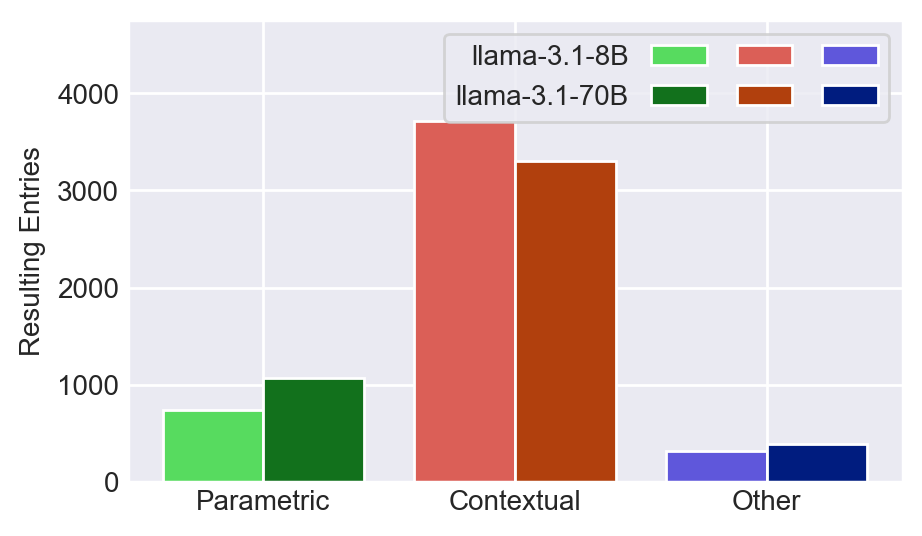
\includegraphics[width=.42\textwidth]{llama_amount.png}
	}
	\caption{Results by type depending on which model; these are the same results as \cref{total_table}.}
	\label{total_results}
\end{figure}

As hypothesised in \cref{intro_models_numbers}, there are vast differences on how the models of different types and sizes act when presented with a context that contradicts their knowledge.
This section contains an overview of the differences, which investigated further in \cref{discussion}.

A similar pattern emerges in most (but not all) of the categories, which can be seen in \cref{llama_cats_table,llama_cats_result,flan_cats_table,flan_cats_result}.

\subsubsection{Calculating the attention of the context and question of each query}
\label{attention_results}

Using the method described in \cref{attention_section}, we can find the attention each model gives, on average, to the tokens in the context part of the query, and how much to the rest.
% The results are present in \cref{attention_table}.

\begin{table}[h]
	\centering
	\scriptsize
	\begin{tabular}{l | r r r r}
		\toprule
			Query Part & \smallflan{} & \bigflan{} & \llamaparbox{} & \bigllamaparbox{} \\
		\midrule
			Context & 0.18 & 0.22 & 0.08 & 0.06 \\
			Rest & 0.03 & 0.05 & 0.03 & 0.01 \\
		\bottomrule
	\end{tabular}
	\caption{Average normalised attention of the query on the tokens corresponding to the context of the query and o the rest. All models pay more attention to the context section of the query than to the rest, but Seq2Seq models tend to have a much higher ratio than decoder-only models.}
	\label{attention_table}
\end{table}

\begin{table}[p]
	\centering
	\footnotesize
	\begin{tabular}{>{\bfseries}l | r r r | r r r}
		\toprule
			& \multicolumn{3}{|c}{\smallflan{}} & \multicolumn{3}{|c}{\bigflan{}} \\
			& \Parametric{} & \Contextual{} & \Other{} & \Parametric{} & \Contextual{} & \Other{} \\
		\midrule
			Person           &  32 &  900 & 37 &  23 &  890 & 56 \\
			City             & 120 & 1030 & 40 &  78 & 1093 & 19 \\
			Principle        &  13 &  164 &  8 &   9 &  168 &  8 \\
			Element          &   6 &  637 &  2 & 102 &  515 & 28 \\
			Book             &  26 &  488 & 25 &  18 &  457 & 64 \\
			Painting         &  26 &  446 & 56 &   4 &  498 & 26 \\
			Historical Event &  11 &  217 & 28 &   1 &  254 &  1 \\
			Building         &  14 &  174 & 10 &   0 &  189 &  9 \\
			Composition      &   0 &  228 & 22 &   7 &  240 &  3 \\
		\bottomrule
	\end{tabular}
	\caption{Results for running each one of the 10 categories separately on the Seq2Seq models. There is not a significant difference between categories.}
	\label{flan_cats_table}
\end{table}

\begin{table}[p]
	\centering
	\footnotesize
	\begin{tabular}{>{\bfseries}l | r r r | r r r}
		\toprule
			& \multicolumn{3}{c|}{\smallllama{}} & \multicolumn{3}{c}{\bigllama{}} \\
			& \Parametric{} & \Contextual{} & \Other{} & \Parametric{} & \Contextual{} & \Other{} \\
		\midrule
			Person           &  40 &  833 & 96 & 209 & 614 & 146 \\
			City             & 117 & 1007 & 66 & 166 & 966 &  58 \\
			Principle        &  44 &  118 & 23 &  44 & 117 &  24 \\
			Element          & 218 &  385 & 42 & 275 & 347 &  23 \\
			Book             & 135 &  344 & 60 & 154 & 318 &  67 \\
			Painting         &  47 &  458 & 23 &  49 & 445 &  34 \\
			Historical Event &  81 &  154 & 21 & 117 & 118 &  21 \\
			Building         &  27 &  163 &  8 &  31 & 159 &   8 \\
			Composition      &  36 &  200 & 14 &  25 & 219 &   6 \\
		\bottomrule
	\end{tabular}
	\caption{Results for running each one of the 10 categories separately on the Decoder-only models, there are a few differences in the results for different categories, which is likely caused by the average answer size.}
	\label{llama_cats_table}
\end{table}

\begin{figure}[p]
	\centering
	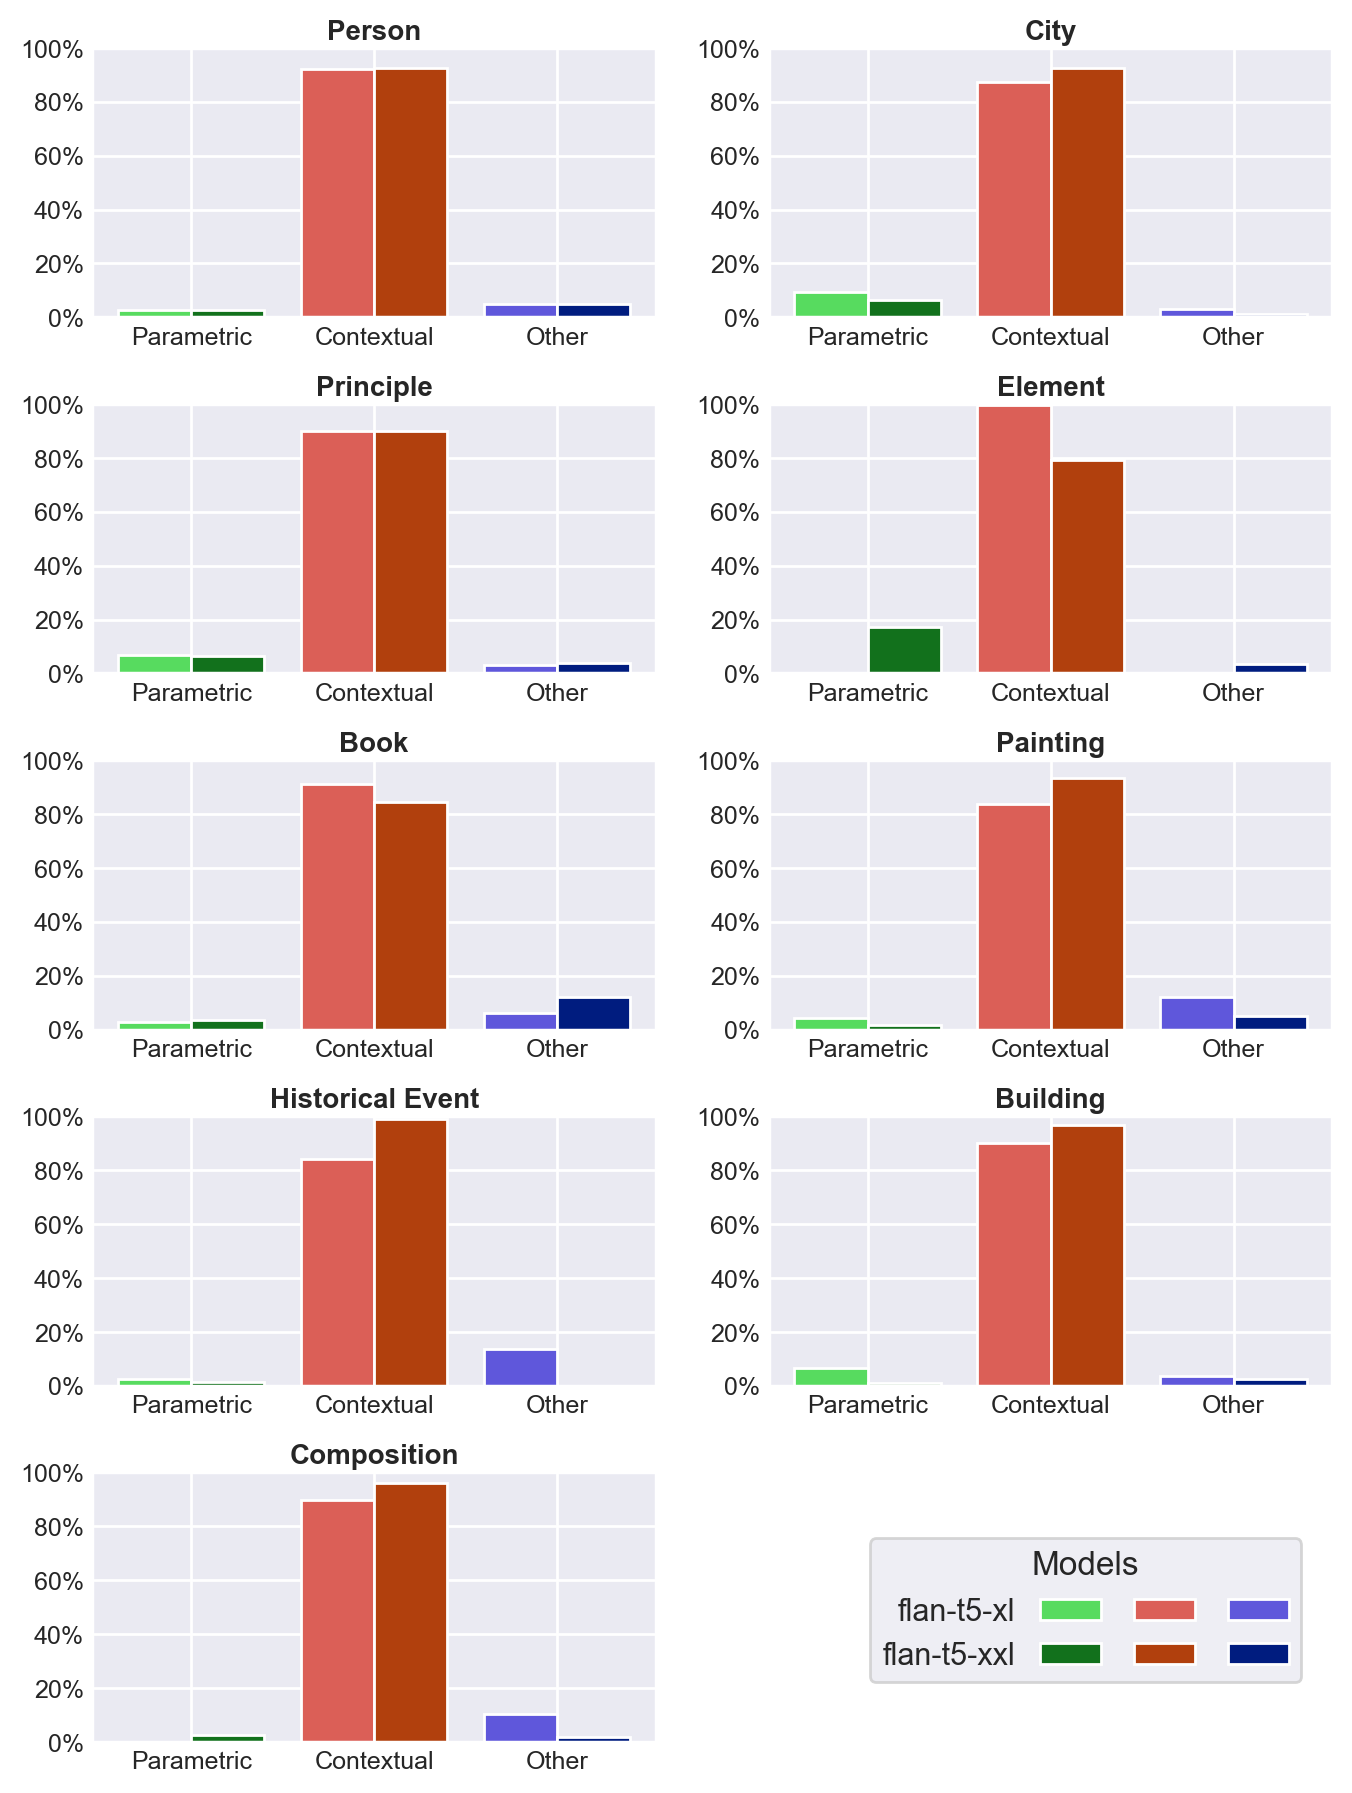
\includegraphics[width=\textwidth]{flan_allcats.png}
	\caption{Results of running Seq2Seq models on the queried data, grouped by category. This plots the information shown in \cref{flan_cats_table}, and we can confirm that there isn't a significant difference in the source of the knowledge used to generate the answer depending on category.}
	\label{flan_cats_result}
\end{figure}

\begin{figure}[p]
	\centering
	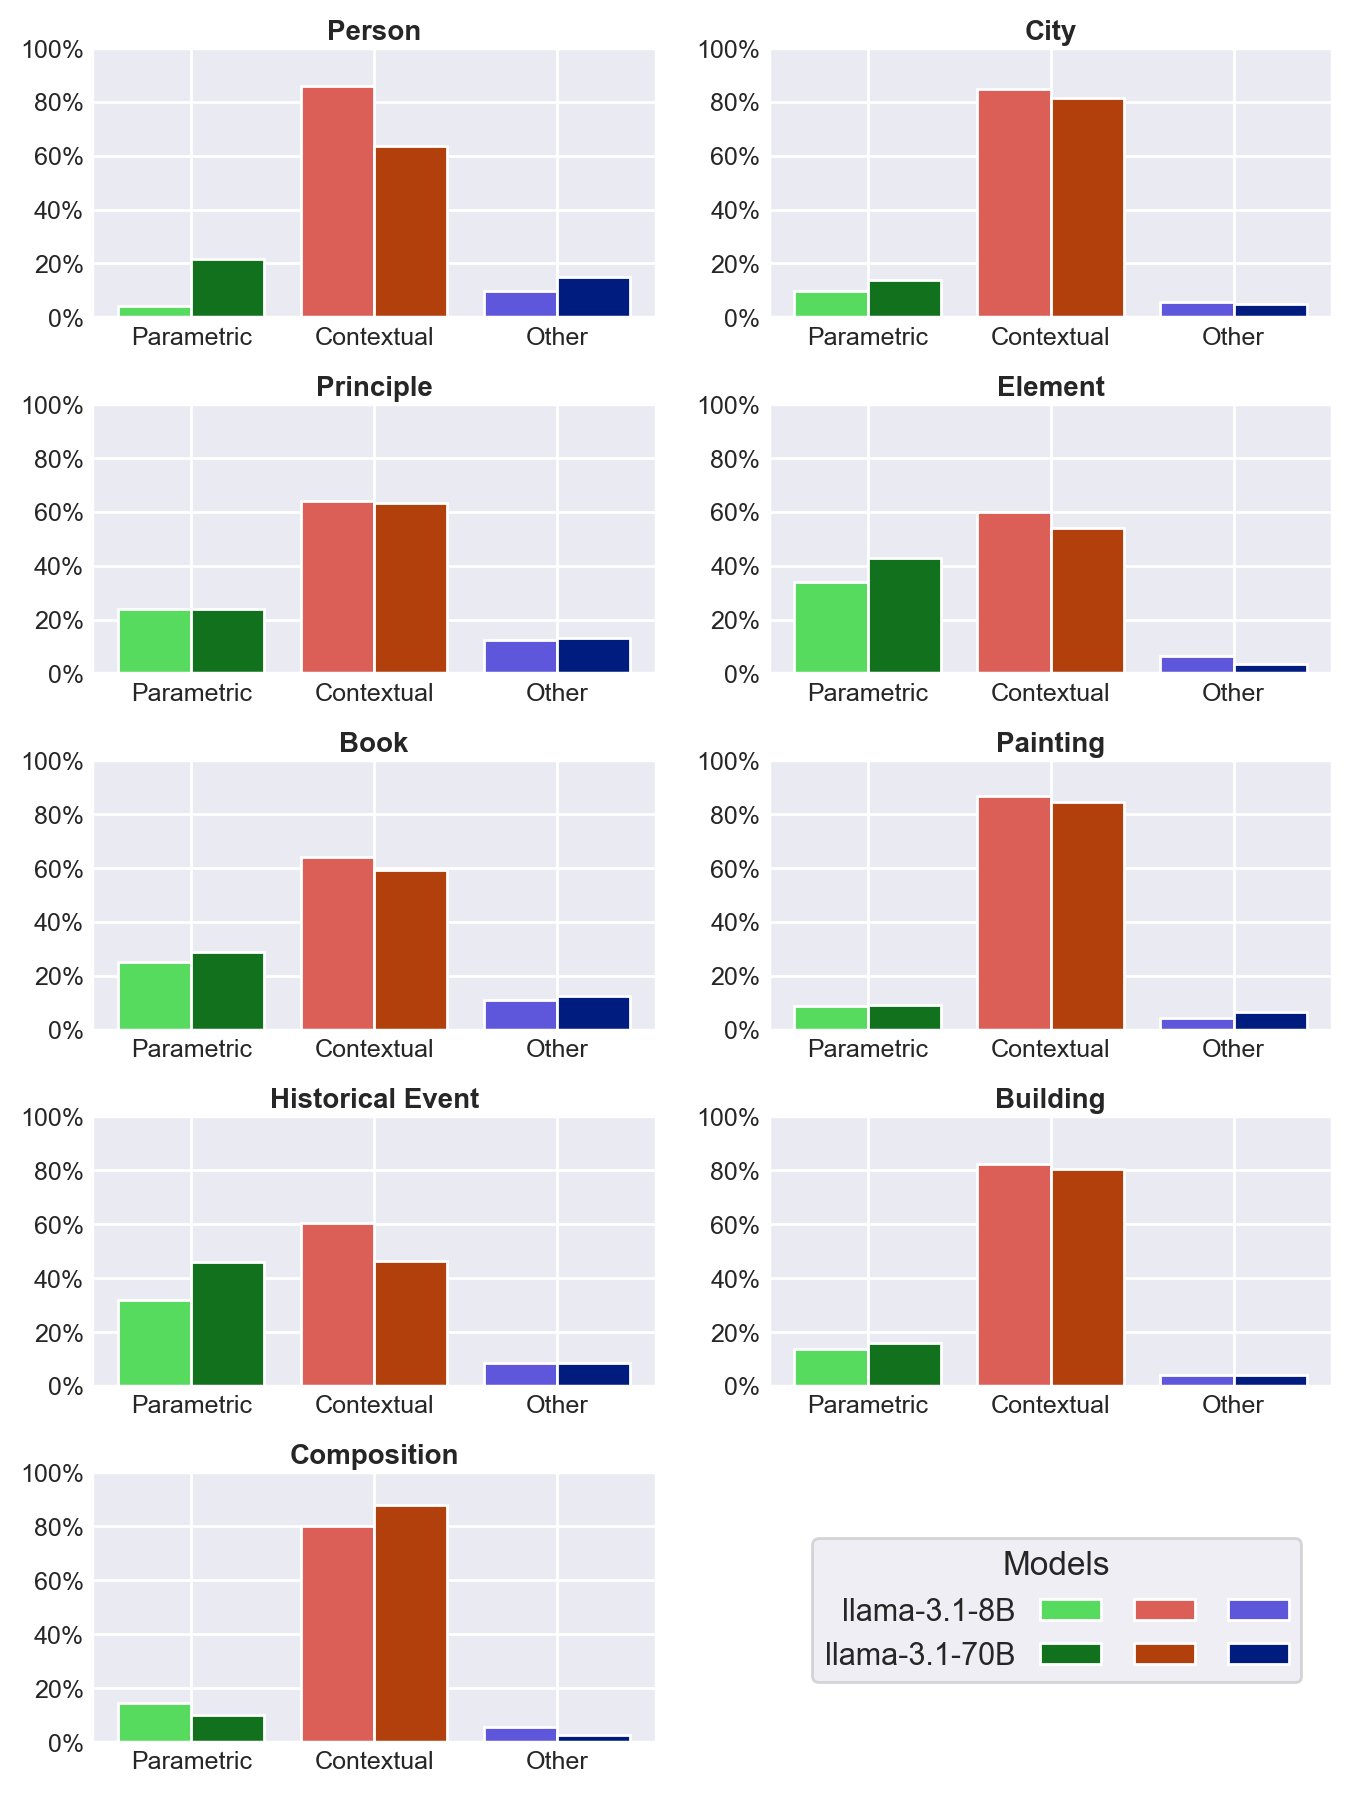
\includegraphics[width=\textwidth]{llama_allcats.png}
	\caption{Results of running decoder-only models on the queried data, grouped by category. This plots the information shown in \cref{llama_cats_table}. Contrasting this to the previous plot, we can see that there is a significant difference in contexts that tend to have questions resulting in shorter answers, such as books and historical events, compared to sections that tend to have longer answers, such as persons.}
	\label{llama_cats_result}
\end{figure}

\clearpage{}
\subsection{Enhancing the framework to understand the reasoning behind each answer}
\label{results_perplexity_score}

We calculate the resulting perplexity of each query as explained in \cref{method_perplexity}.
These are accumulated in three distributions, depending on answer type, which are summarised in \cref{perplexity_flan_table,perplexity_llama_table,perplexity_results}, and grouped by different categories in \cref{flan_catboxes,llama_catboxes}, and later grouped by category in \cref{flan_catboxes,llama_catboxes}.

\begin{table}[ht]
	\centering
	\scriptsize
	\begin{tabular}{>{\bfseries}l | r r | r r}
		\toprule
			& \multicolumn{2}{|c}{\smallflan} & \multicolumn{2}{|c}{\bigflan} \\
			& \Parametric{} & \Contextual{} & \Parametric{} & \Contextual{} \\
		\midrule
			count & 588 & 4172 & 491 & 4269 \\
			mean & 7.02 & 1.55 & 12.01 & 1.24 \\
			std & 11.25 & 0.56 & 18.91 & 0.68 \\
			10\% & 2.60 & 1.08 & 1.47 & 1.00 \\
			25\% & 3.21 & 1.18 & 2.54 & 1.02 \\
			50\% & 4.71 & 1.37 & 4.00 & 1.08 \\
			75\% & 7.40 & 1.69 & 8.37 & 1.22 \\
			90\% & 10.72 & 2.32 & 44.25 & 1.54 \\
		\bottomrule
	\end{tabular}
	\caption{Distribution of perplexity values for Seq2Seq models. The perplexity of \Parametric{} answers is consistently higher than the one of \Contextual{} answers.}
	\label{perplexity_flan_table}
\end{table}

\begin{table}[ht]
	\centering
	\scriptsize
	\begin{tabular}{>{\bfseries}l | r r | r r}
		\toprule
			& \multicolumn{2}{|c}{\smallllama} & \multicolumn{2}{|c}{\bigllama} \\
			& \Parametric{} & \Contextual{} & \Parametric{} & \Contextual{} \\
		\midrule
			count & 289 & 4471 & 383 & 4377 \\
			mean & 1.64 & 1.20 & 1.56 & 1.22 \\
			std & 0.87 & 0.30 & 0.46 & 0.31 \\
			10\% & 1.18 & 1.03 & 1.20 & 1.03 \\
			25\% & 1.28 & 1.05 & 1.28 & 1.06 \\
			50\% & 1.45 & 1.11 & 1.43 & 1.12 \\
			75\% & 1.72 & 1.23 & 1.68 & 1.25 \\
			90\% & 2.22 & 1.43 & 2.04 & 1.49 \\
\bottomrule
	\end{tabular}
	\caption{Distribution of perplexity values for Decoder-only models. The same differences in \cref{perplexity_flan_table} appear here, but to a lesser degree.}
	\label{perplexity_llama_table}
\end{table}

\begin{figure}[H]
	\centering
	\subfigure[Seq2Seq models]{
		\raggedleft
		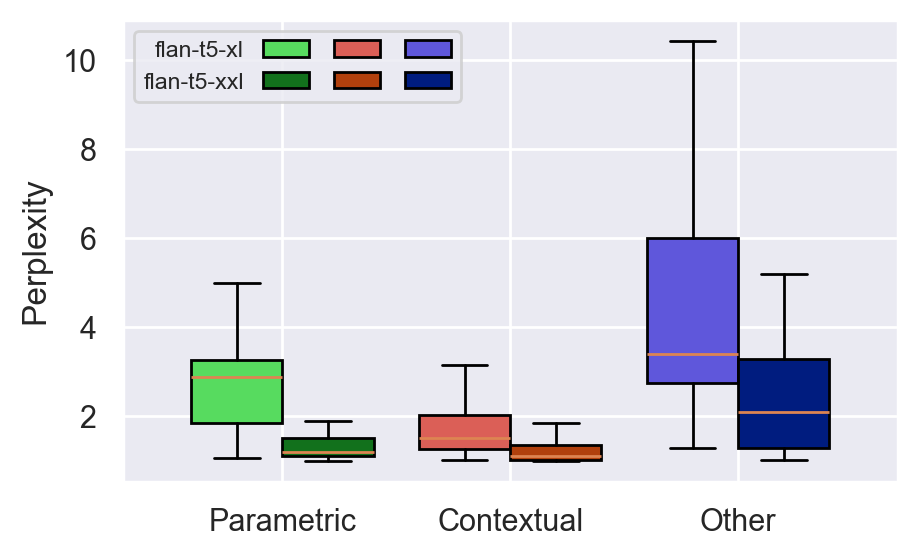
\includegraphics[width=.48\textwidth]{flan_boxplot.png}
	}%
	\subfigure[Decoder-only models]{
		\raggedright
		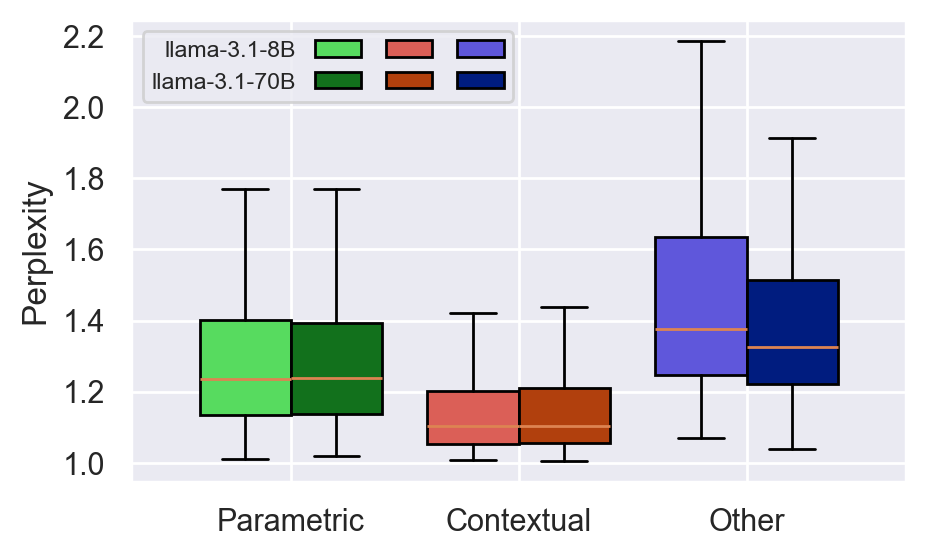
\includegraphics[width=.48\textwidth]{llama_boxplot.png}
	}
	\caption{Perplexity distribution according to model architecture and size. These represent the same distributions as \cref{perplexity_llama_table,perplexity_flan_table}.}
	\label{perplexity_results}
\end{figure}

\begin{figure}[p]
	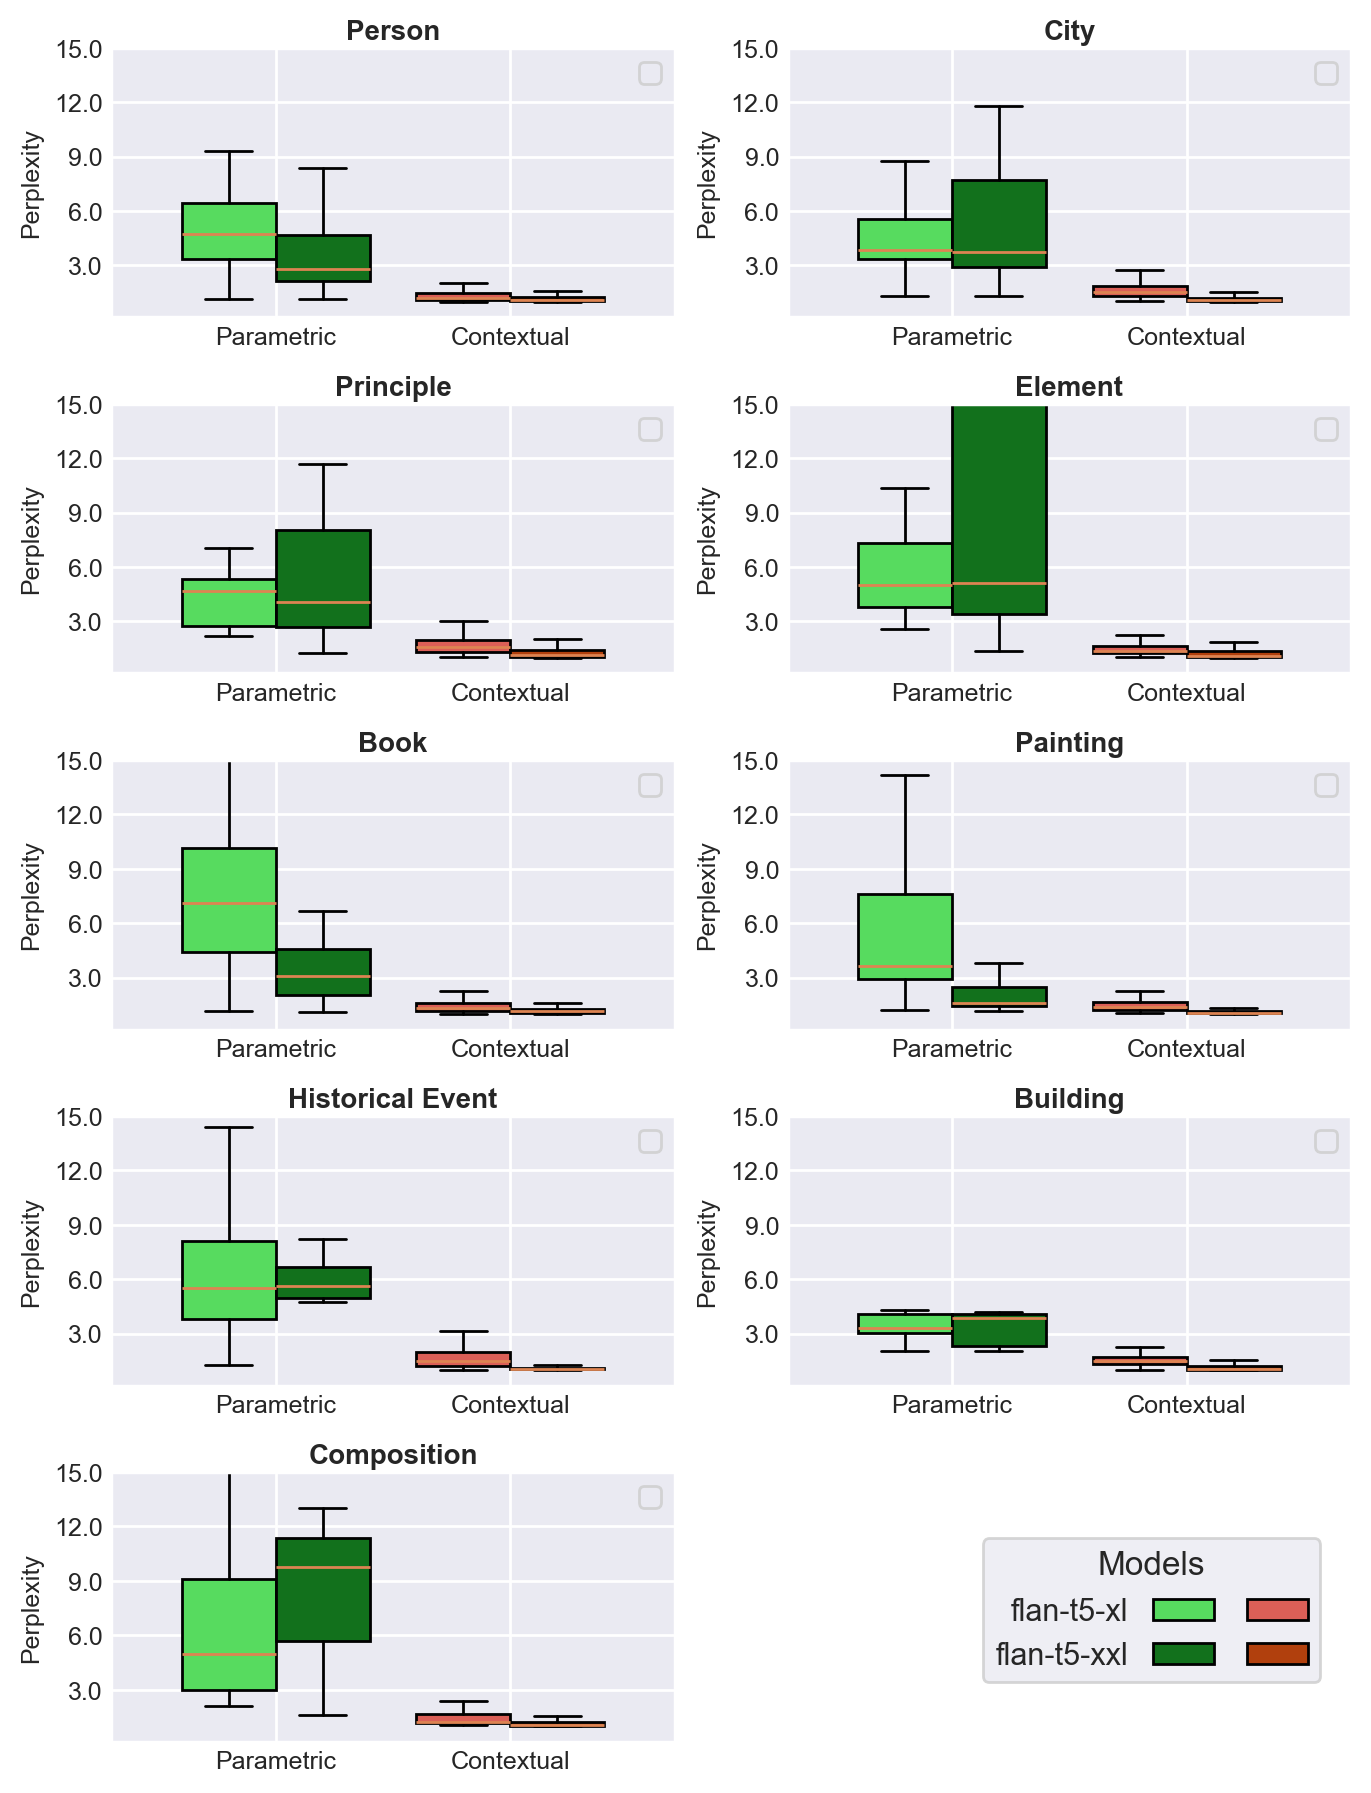
\includegraphics[width=\textwidth]{flan_catboxes.png}
	\caption{Box plots representing the distribution of the perplexities when running both Flan-T5 models, grouped by category. There are considerable differences in the distribution of perplexity values for \Parametric{} answers, but not so much for \Contextual{} answers. Still, the differences between this two are consistently large.}
	\label{flan_catboxes}
\end{figure}

\begin{figure}[p]
	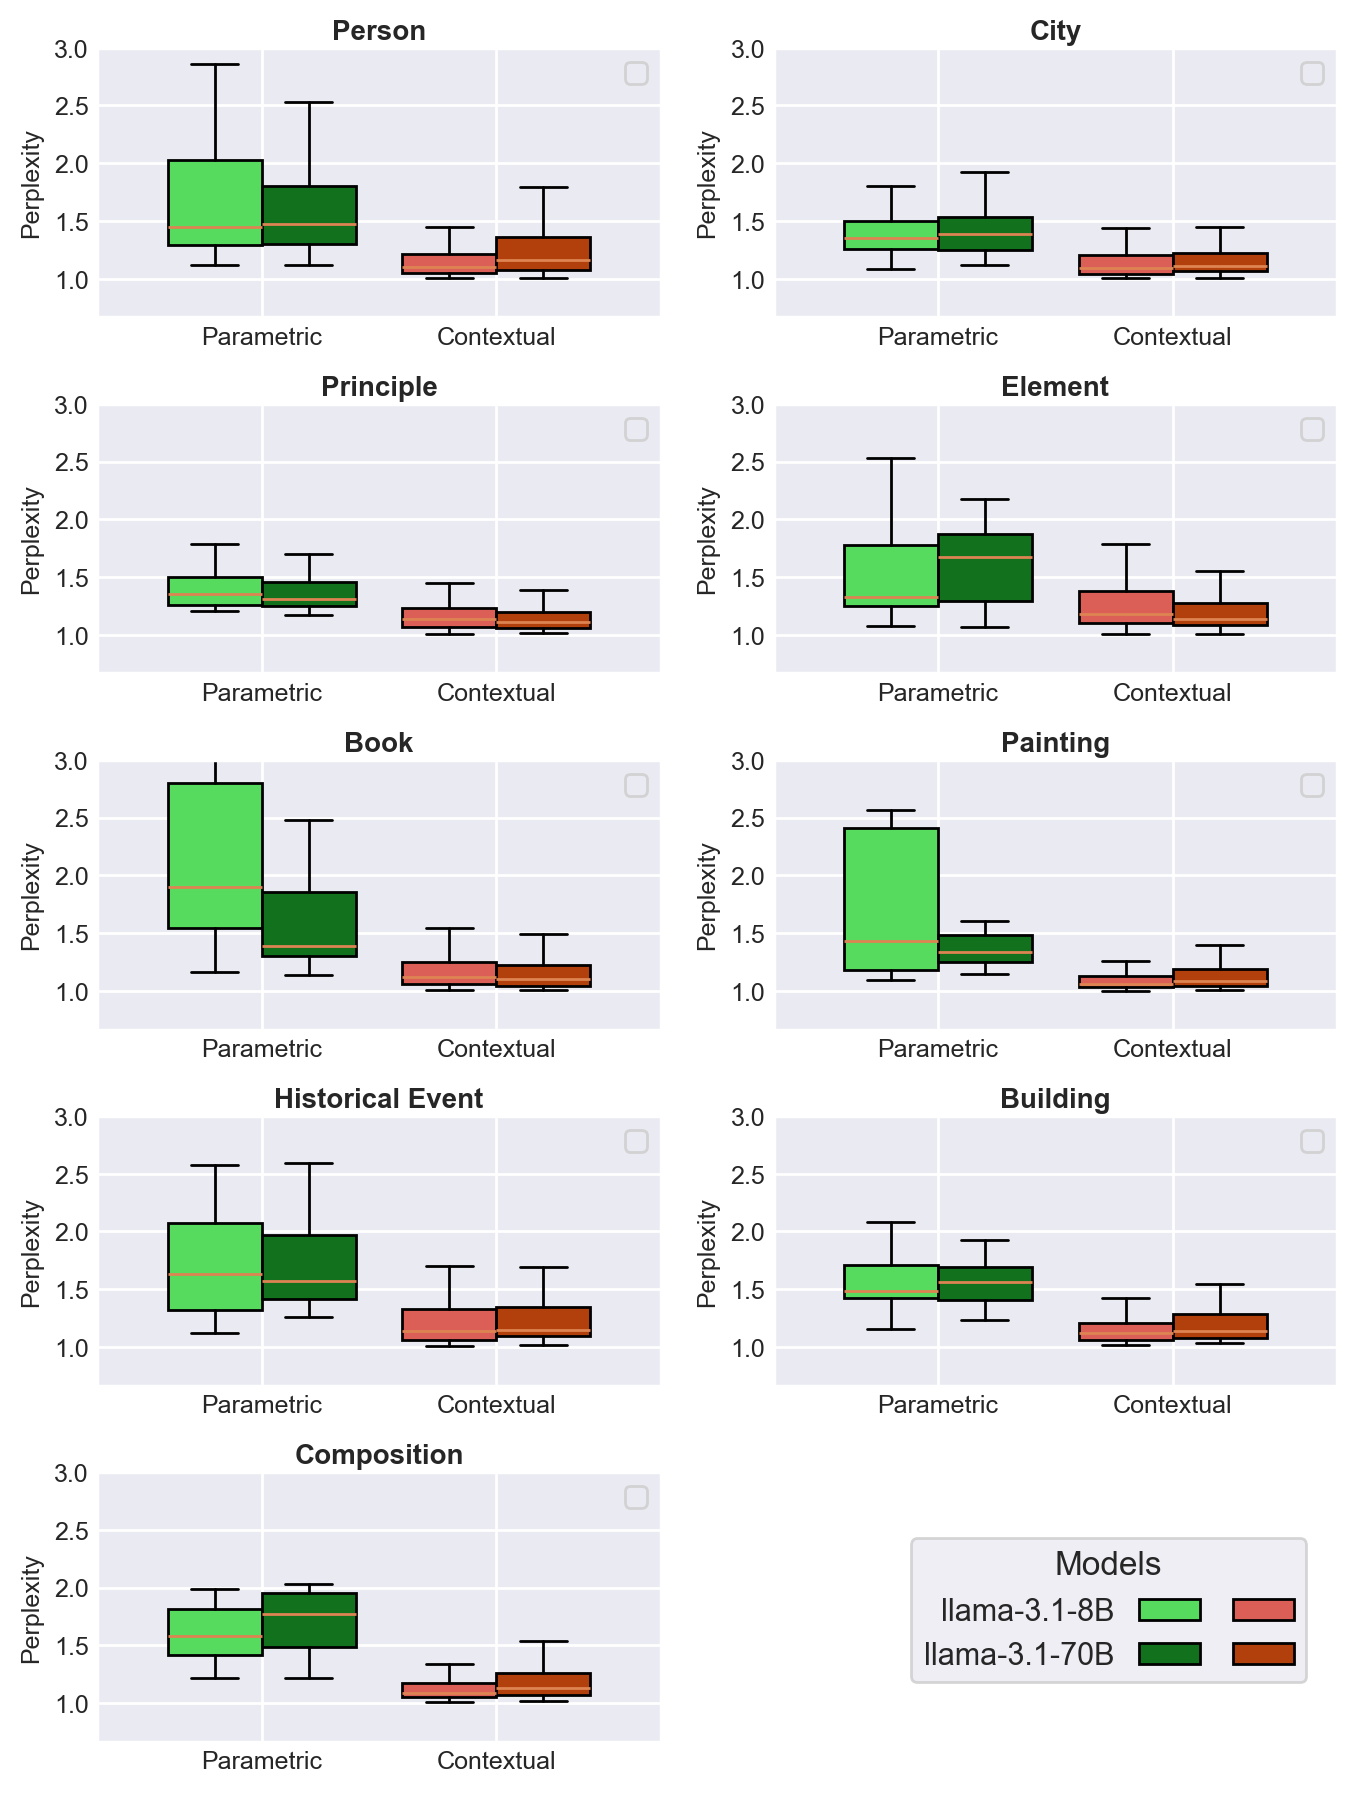
\includegraphics[width=\textwidth]{llama_catboxes.png}
	\caption{Box plots representing the distribution of the perplexities when running both Llama models, grouped by category. The entire distribution of perplexities is much smaller, and the differences in these for \Paramteric{} answers are less variable as in the previous plots for Seq2Seq models.}
	\label{llama_catboxes}
\end{figure}
